\documentclass[12pt,letterpaper]{article}

\newenvironment{proof}{\noindent{\bf Proof:}}{\qed\bigskip}

\newtheorem{theorem}{Theorem}
\newtheorem{corollary}{Corollary}
\newtheorem{lemma}{Lemma} 
\newtheorem{claim}{Claim}
\newtheorem{fact}{Fact}
\newtheorem{definition}{Definition}
\newtheorem{assumption}{Assumption}
\newtheorem{observation}{Observation}
\newtheorem{example}{Example}
\newcommand{\qed}{\rule{7pt}{7pt}}

\newcommand{\assignment}[4]{
\thispagestyle{plain} 
\newpage
\setcounter{page}{1}
\noindent
\begin{center}
\framebox{ \vbox{ \hbox to 6.28in
{\bf CS578/STAT590: Introduction Machine Learning \hfill #1}
\vspace{4mm}
\hbox to 6.28in
{\hspace{2.5in}\large\mbox{Problem Set #2}}
\vspace{4mm}
\hbox to 6.28in
{{\it Handed Out: #3 \hfill Due: #4}}
}}
\end{center}
}

\newcommand{\solution}[4]{
\thispagestyle{plain} 
\newpage
\setcounter{page}{1}
\noindent
\begin{center}
\framebox{ \vbox{ \hbox to 6.28in
{\bf CS578/STAT590: Introduction to Machine Learning \hfill #4}
\vspace{4mm}
\hbox to 6.28in
{\hspace{2.5in}\large\mbox{Problem Set #3}}
\vspace{4mm}
\hbox to 6.28in
{#1 \hfill {\it Handed In: #2}}
}}
\end{center}
\markright{#1}
}

\newenvironment{algorithm}
{\begin{center}
\begin{tabular}{|l|}
\hline
\begin{minipage}{1in}
\begin{tabbing}
\quad\=\qquad\=\qquad\=\qquad\=\qquad\=\qquad\=\qquad\=\kill}
{\end{tabbing}
\end{minipage} \\
\hline
\end{tabular}
\end{center}}

\def\Comment#1{\textsf{\textsl{$\langle\!\langle$#1\/$\rangle\!\rangle$}}}



\oddsidemargin 0in
\evensidemargin 0in
\textwidth 6.5in
\topmargin -0.5in
\textheight 9.0in

\begin{document}

\solution{Gen Nishida}{\today}{1}{Fall 2014}
% Fill in the above, for example, as follows:
% \solution{John Smith}{\today}{1}{Fall 2014}

\pagestyle{myheadings}  % Leave this command alone

\section{Review Questions}

\begin{enumerate}
\item Assume the probability of getting {\it head} when tossing a coin is $\lambda$.
\begin{itemize}
\item What is the probability of getting the first head at the (k+1)-th toss?
\[
(1-\lambda)^k \lambda
\]
\item What is the expected number of tosses needed to get the first head?\\
Let $k$ be the number of tosses needed to get the first head. Then the expected number of $k$ is defined by
\begin{eqnarray}
E[k]&=&\lambda \times 1 + (1-\lambda) \lambda \times 2 + (1-\lambda)^2 \lambda \times 2 + \cdots\\
(1-\lambda)E[k]&=&(1-\lambda)\lambda + (1-\lambda)^2 \lambda \times 2 + (1-\lambda)^3 \lambda \times 3 + \cdots
\end{eqnarray}
By subtracting (2) from (1), we get
\begin{eqnarray*}
\lambda E[k] &=& \lambda + (1-\lambda) \lambda + (1-\lambda)^2 \lambda + (1-\lambda)^3 \lambda + \cdots\\
 &=&\lambda \frac{1}{1 - (1 - \lambda)}\\
 &=&1 .
\end{eqnarray*}
Thus, $E[k]=1 / \lambda $.
\end{itemize}

\item Let $f(x, y)=3x^2+y^2-xy-11x$

\begin{itemize}
\item What is the partial derivative of $f$ with respect to $x$ $(\frac{\partial f}{\partial x})$? Find $\frac{\partial f}{\partial y}$ as well.
\[
\frac{\partial f}{\partial x}=6x-y-11,\:\:  \frac{\partial f}{\partial y}=2y - x
\]
\item Find a point $(x, y)$ that minimizes $f$.
\[
\left\{
\begin{array}{l}
6x-y-11=0 \\
2y-x=0
\end{array}
\right.
\]
By solving these equations, we get $(x, y)=(2, 1)$.
\end{itemize}

\item 
\begin{itemize}
\item Assume that $\omega \in R^n$ and $b$ is a scalar. A hyperplane in $\mathbb{R}^n$ is the set $\{x : x\in \mathbb{R}^n, \omega^Tx+b=0\}$. For $n=2$ and $n=3$, draw on paper an example of a hyperplane.\\
The hyperplane has it normal vector $\omega$, and it is away from the origin by $-b/\|\omega\|$. The example of a hyperplane for $n=2$ and $n=3$ is shown in Figure \ref{fig:one}.

\begin{figure}[hbtp]
\centering
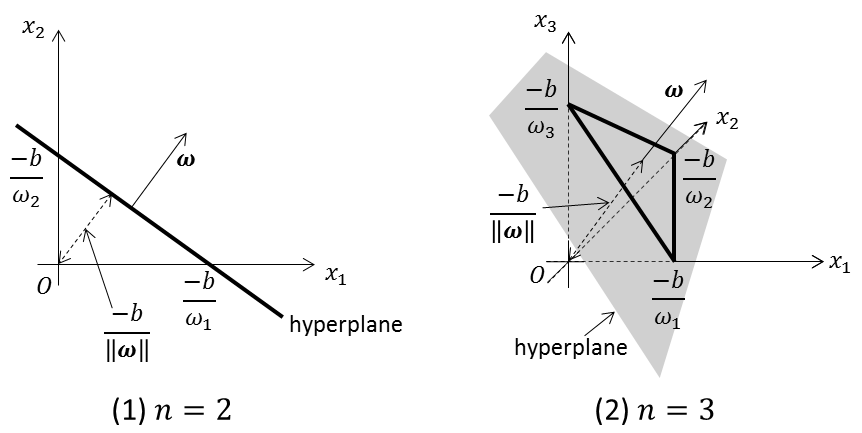
\includegraphics[width=130mm]{figure1.png}
\caption{The example of a hyperplane}
\label{fig:one}
\end{figure}


\item Assume we have two parallel hyperplanes: $\{x: x\in \mathbb{R}^n, \omega^Tx+b_1=0\}$ and $\{x: x\in \mathbb{R}^n, \omega^Tx+b_2=0\}$. What is the distance between these two hyperplanes?
\[
\left|\frac{-b_1}{\|\omega\|}-\frac{-b_2}{\|\omega\|}\right|=\frac{|b_1-b_2|}{\|\omega\|}
\]
\end{itemize}
\end{enumerate}

\section{Basic Concepts}
\begin{enumerate}
\item Define in one sentence: (1) training set, (2) test set, (3) validation set. Your definition should use the notation described in class.
\begin{itemize}
\item training set

Training set $S_{ts}$ is a set of data $(x, y) \in S_{ts}$, where $x$ is a instance and $y$ is a label, which is used to optimize a hypothesis function $f$ by increasing the accuracy $\Pr(f(x)=y)$.

\item test set

Test set $S_{ts}$ is a set of data $(x, y) \in S_{ts}$, where $x$ is a instance, $y$ is a label, and $S_{ts} \cap S_{tr} = \phi$, which is used to compute $\Pr(f(x)=y)$ as the performance of the hypothesis $f$.

\item validation set

Validation set $S_{v}$ is a set of data $(x, y) \in S_{v}$, where $x$ is a instance, $y$ is a label, $S_{v} \cap S_{tr} = \phi$, and $S_{v} \cap S_{ts} = \phi$, which is used to estimate the performance of the hypothesis $f$ by computing $\Pr(f(x)=y)$ and to generalize $f$ preventing from overfitting the training data.

\end{itemize}

\item Can you use the validation set as a test set?

No. The validation set has to be disjoint from the test set. Since validation set is used to estimate the accuracy of the hypothesis during the training phase, the resulting hypothesis is optimized for the validation set, and it is meaningless to use the validation set as a test set in order to measure the actual performance of the hypothesis.

\item Define in one sentence: overfitting

A hypothesis $f$ is said to overfit the training data $(x_{tr}, y_{tr}) \in S_{tr}$ if it has smaller error $e_{tr} = 1 - \Pr(f(x_{tr})=y_{tr})$ on the training data but loses the generalization performance and has larger error $e_{ts} = 1 - \Pr(f(x_{ts})=y_{ts})$ on test data $(x_{ts}, y_{ts}) \in S_{ts}$.

\item True or False (and why): A learned hypothesis $f$ has a training error $e_{tr}$ and a testing error $e_{ts}$, where $e_{tr} > e_{ts}$.

\begin{itemize}
\item (1) can we say that $f$ overfits to the training data?

False. Since the hypothesis $f$ is optimized for the training data while the test data is unknown during training phase, the training error $e_{tr}$ is smaller than $e_{ts}$ in general, even if $f$ is well generalized. In this case, $e_{tr} > e_{ts}$, which indicates that $e_{ts}$ is very small and $f$ is generalized very well in this sense.

\item (2) Now, assume that $e_{tr} < e_{ts}$, does $f$ overfit to the training data?

False. Since the hypothesis $f$ is optimized for the training data while the test data is unknown during training phase, the training error $e_{tr}$ is smaller than $e_{ts}$ in general, even if $f$ is well generalized. The optimal hypothesis minimizes $e_{ts}$, but still it might be the case that $e_{tr} < e_{ts}$. Therefore, we cannot conclude that $f$ overfits the training data even if $e_{tr} < e_{ts}$, unless we find another hypothesis $f'$ which has larger error on the training data but smaller error on the test data compared to $f$.

\end{itemize}

\end{enumerate}

\section{Decision Trees}

\begin{enumerate}
\item The "Thrill and Romance" bookstore

\begin{itemize}
\item What is the entropy of the target variable? (Buy)

The number of examples labeled "Buy=Y" is 7, while the number of examples labeled "Buy=N" is 4. Thus,
\[
-\frac{7}{11}\log \frac{7}{11}-\frac{4}{11}\log \frac{4}{11}=0.94566
\]

\item What are the attributes considered by the algorithm?

All the attributes, "Pages", "Famous Author", "Category", and "Cover Color" should be considered by the algorithm. For "Pages", since it is a continuous attribute, we first have to sort examples according to the values of "Pages" and check the mid-point as a possible threshold in order to discretize. The sorted values are as follows:\\
45(-), 50(+), 72(+), 100(-), 120(+), 142(+), 150(+), 200(-), 300(+), 350(+), 1000(-).\\
Thus, the possible thresholds for "Pages" are 47.5, 86, 110, 175, 250, and 675. These thresholds are called cut points \cite{fayyad1992}, and used to split the continuous space into two ranges so that the continuous values can be handled in the same manner with the discrete values. Note that the thresholds have to be calculated for every node, since the set of the continuous values for each node may differ from the root node.

\item What is the first attribute that the algorithm will split the data on? What is its information gain?

The information gain by the split of each attribute is computed as follows.

\begin{itemize}
\item Pages(threshold=47.5)
\begin{eqnarray*}
0.94566 - \left[ 0 \times \frac{1}{11} - \left( -\frac{7}{10} \log \frac{7}{10} - \frac{3}{10} \log \frac{3}{10} \right) \times \frac{10}{11}  \right]\\ = 0.94566 - 0.80117 = 0.14449
\end{eqnarray*}
\item Pages(threshold=86)
\begin{eqnarray*}
0.94566 - \left[ \left( -\frac{2}{3} \log \frac{2}{3} -\frac{1}{3} \log \frac{1}{3} \right) \times \frac{3}{11} + \left( -\frac{5}{8} \log \frac{5}{8} - \frac{3}{8} \log \frac{3}{8} \right) \times \frac{8}{11} \right]\\ = 0.94566 - 0.94458 = 0.00108
\end{eqnarray*}
\item Pages(threshold=110)
\begin{eqnarray*}
0.94566 - \left[ 1.0 \times \frac{4}{11} - \left( -\frac{5}{7} \log \frac{5}{7} - \frac{2}{7} \log \frac{2}{7} \right) \times \frac{7}{11}  \right]\\ = 0.94566 - 0.91289 = 0.03277
\end{eqnarray*}
\item Pages(threshold=175)\\
Same as threshold=110, which is 0.03277.
\item Pages(threshold=250)\\
Same as threshold=86, which is 0.00108.
\item Pages(threshold=675)\\
Same as threshold=47.5, which is 0.14449.
\item Famous Author
\begin{eqnarray*}
0.94566 - \left[ \left( -\frac{5}{7} \log \frac{5}{7} -\frac{2}{7} \log \frac{2}{7} \right) \times \frac{7}{11} + 1.0 \times \frac{4}{11} \right]\\ = 0.94566 - 0.91289 = 0.03277
\end{eqnarray*}
\item Category
\begin{eqnarray*}
0.94566 - \left[ \left( -\frac{4}{5} \log \frac{4}{5} -\frac{1}{5} \log \frac{1}{5} \right) \times \frac{5}{11} + 1.0 \times \frac{6}{11} \right]\\ = 0.94566 - 0.8736 = 0.07206
\end{eqnarray*}
\item Cover Color
\begin{eqnarray*}
0.94566 - \left[ \left( -\frac{6}{9} \log \frac{6}{9} -\frac{3}{9} \log \frac{3}{9} \right) \times \frac{9}{11} + 1.0 \times \frac{2}{11} \right]\\ = 0.94566 - 0.93315 = 0.01251
\end{eqnarray*}
\end{itemize}
The attribute which achieves the highest information gain is "Pages" with 47.5 or 675 as the threshold, so we should use "Pages" as the first attribute to split, and the information gain is 0.14449.
Note that if we split all the values of "Pages", then we will be able to completely separate the labels with the weighted averaged of the entropy = 0.0. However, this will be overfitting, and we do not want to do that.

\item Due to a computer error some of the training examples attributes were deleted! Revise the decision tree training algorithm to deal with missing values in the training data.

The goal of training is to minimize the expected loss over the distribution of values of attributes. Intuitively, it is better to use this distribution to estimate the missing values, but, we do not know the distribution in advance. One option would be to choose the majority votes for the missing values. Suppose the first row in our training data does not have a value of "Famous Author". If we use "Famous Author" as the first attribute to split the tree, then we assign "Y" for the first row, becuase "Y" is the majority. Although this options is easy to implement, the minority values may be ignored during the decision tree building.

Another option is to use the probability distribution according to the training data. If we have enough number of training data without missing values, the distribution of the values in the training data is likely to be similar to the one of testing data. Hence, it is reasonable to use the distribution of the values in the training data to estimate the missing values. In the same example above, in which the first row of the training data has missing value for "Famous Author", we get "Y" with probability 0.6 and "N" with probability 0.4. Based on this, the first row contributes 0.6 to the sub-tree for "Y", while it contirbutes 0.4 to the other sub-tree for "N". In the decision tree implementation in the following section, I used the latter approach.
\end{itemize}

\item Decision Tree Implementation

I implemented the decision tree algorithm using the second option for the missing values. With regard to the continuous values, for every node, I computed the expected information gain for each cut point discussed above in addition to the discrete attributes, and choose the best one which achieves the highest information gain. Also, the validation data was used to find the best maxDepth, changing from 0 to 20. Finally, the performance of the resulting decision tree was measured on the test data. Please refer to the attached source code for details.

\begin{table}[htb]
\begin{center}
\caption{Results}
\begin{tabular}{|c|c|c|} \hline
maxDepth & Validation data & Test data \\ \hline \hline
0 & 0.58461 & 0.50746 \\ \hline
1 & 0.96923 & 0.52238 \\ \hline
2 & 0.96923 & 0.52238 \\ \hline
3 & 0.96923 & 0.52238 \\ \hline
4 & 0.90769 & 0.56716 \\ \hline
5 & 0.92307 & 0.56716 \\ \hline
6 & 0.92307 & 0.56716 \\ \hline
7 & 0.92307 & 0.56716 \\ \hline
8 & 0.92307 & 0.56716 \\ \hline
9 & 0.92307 & 0.56716 \\ \hline
\end{tabular}
\label{tab:result}
\end{center}
\end{table}

The results of my decision tree on the validation and testing data are shown in Table \ref{tab:result}. Since the testing data is not available beforehand, we have to choose the best maxDepth only based on the results on the validation data. Thus, we choose $maxDepth=1$, and we get 0.52238 as the accuracy on the test data. Note that this result is better than the case of $maxDepth=0$, which is a baseline, but there is significant difference in the accuracy between the results on validation and training data.

This poor performance is caused by the different distribution of values in the feature space between the training data and the test data. To investigate more details, I computed the distribution of labels in the child nodes of the root node as shown in Figure \ref{fig:comparison}. The results indicate that the distribution of the values of 9th attribute against the labels is significantly different between the training data and the test data. In the training data, most data with the value "t" for the 9th attribute have positive labels, while most data with the value "f" for the 9th attribute have negative labels. This polarization leads to low entropy, i.e. high information gain. In the test data, on the other hand, both subsets have both labels almost evenly, which results in very high entroy, i.e. low information gain. Hence, the decision tree trained from the training data could not get high accuracy on the test data.

\begin{figure}[hbtp]
\centering
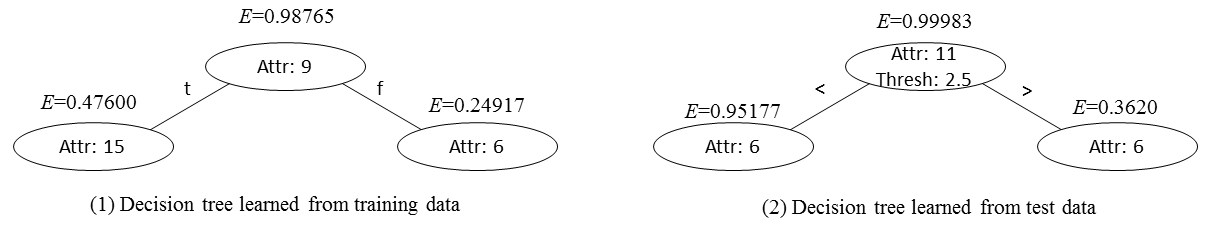
\includegraphics[width=150mm]{figure2.png}
\caption{Comparison of the entropy between the training data and the test data: The splitting by the 9th attribute on the training data achieves very low entroy, whose weighted average is 0.35332. This is why the 9th attribute was selected as the root node for the decision treee. On the other hand, the splitting by the same attribute on the test data results in very high entroy, whose weighted average is 0.99671. This indicates that the distribution of the 9th values against the labels are significantly different between the training data and the test data, and this causes very poor performance of the decision tree on the test data.}
\label{fig:comparison}
\end{figure}

\end{enumerate}

\begin{thebibliography}{9}
\bibitem{fayyad1992} Fayyad, Usama M. and Irani, Keki B. 1992. On the Handling of Continuous-Valued Attributes in Decision Tree Generation. {\it Machine Learning}, 8, pp. 87 - 102.
\end{thebibliography}

\end{document}

